% unit: u18
% sources: sources/097-projection-matrices-and-least-squares.txt, sources/030-lecture-16-projection-matrices-and-least-squares.txt, sources/179-mit18-06scf11-ses2-3sum-pdf-download-file.txt, sources/031-problem-solving-least-squares-approximation.txt, sources/180-mit18-06scf11-ses2-3prob-pdf-download-file.txt, sources/181-mit18-06scf11-ses2-3sol-pdf-download-file.txt
\section{Projection matrices and least squares}\label{sec:u18}

This section puts the projection formulas of Section~\ref{sec:u17} to work on their most
important application: fitting a straight line to data that no line passes through exactly.
First we look once more at what $P=A(A\T A)^{-1}A\T$ does to the two kinds of vectors it can
meet, because that explains the whole least-squares picture: $\vb{b}$ splits into a part
$\vb{p}$ that the model can explain and an error $\vb{e}$ that it cannot, at right angles.

\subsection{What a projection does to \texorpdfstring{$\vb{b}$}{b}}

\begin{proposition}[The two extreme cases]\label{prop:u18-extremes}
Let $A$ have independent columns and $P=A(A\T A)^{-1}A\T$.
If $\vb{b}\in\Col{A}$ then $P\vb{b}=\vb{b}$; if $\vb{b}\in\Nul{A\T}$ (perpendicular to the
column space) then $P\vb{b}=\vb{0}$.
\end{proposition}

\begin{proof}
A vector in the column space has the form $\vb{b}=A\vb{x}$, and then
$P\vb{b}=A(A\T A)^{-1}(A\T A)\vb{x}=A\vb{x}=\vb{b}$. A vector in $\Nul{A\T}$ has
$A\T\vb{b}=\vb{0}$, and the last factor of $P$ kills it.
\end{proof}

A typical $\vb{b}$ is neither: it has a component in $\Col{A}$ and a component in $\Nul{A\T}$
(Section~\ref{sec:u16}), and the projection keeps the first and kills the second.

\begin{proposition}[The complementary projection]\label{prop:u18-iminusp}
$I-P$ is the projection matrix onto $\Nul{A\T}$: it is symmetric, $(I-P)^2=I-P$, and
$\vb{b}=P\vb{b}+(I-P)\vb{b}=\vb{p}+\vb{e}$ with $\vb{p}\in\Col{A}$, $\vb{e}\in\Nul{A\T}$.
\end{proposition}

\begin{proof}
$(I-P)\T=I-P\T=I-P$, and $(I-P)^2=I-2P+P^2=I-P$ because $P^2=P$. The vector
$(I-P)\vb{b}=\vb{b}-A\hat{\vb{x}}=\vb{e}$ satisfies $A\T\vb{e}=\vb{0}$ by the normal equations,
so it lies in $\Nul{A\T}$. By Proposition~\ref{prop:u18-extremes}, $I-P$ fixes vectors of
$\Nul{A\T}$ and kills vectors of $\Col{A}$; so it is the projection onto $\Nul{A\T}$.
\end{proof}

\subsection{Fitting a line: the least-squares problem}

We are given three measurements $(t,b)=(1,1),\,(2,2),\,(3,2)$ and want the line $b=C+Dt$
that comes closest. If the line went through all three points we would have
\[
  \begin{aligned}
    C+D&=1\\ C+2D&=2\\ C+3D&=2
  \end{aligned}
  \qquad\text{i.e.}\qquad
  \underbrace{\begin{bmatrix}1&1\\1&2\\1&3\end{bmatrix}}_{A}
  \underbrace{\begin{bmatrix}C\\D\end{bmatrix}}_{\vb{x}}
  =\underbrace{\begin{bmatrix}1\\2\\2\end{bmatrix}}_{\vb{b}} .
\]
The first two equations force $C=0$, $D=1$, and then the third fails ($3\neq 2$). Three
equations, two unknowns, no solution: $\vb{b}$ is not in the plane $\Col{A}$. Any choice of
$C,D$ misses by the vector $A\vb{x}-\vb{b}$, whose components are the misses at the three data
points.

\begin{definition}[Least-squares solution]\label{def:u18-ls}
A \emph{least-squares solution} of $A\vb{x}=\vb{b}$ is a vector $\hat{\vb{x}}$ that minimizes
the total squared error
\[
  E(\vb{x})=\|A\vb{x}-\vb{b}\|^2=e_1^2+e_2^2+\cdots+e_m^2 .
\]
Fitting a line this way is called \emph{linear regression}.
\end{definition}

There are two pictures of the same computation, and it pays to keep both. In the
\emph{data picture} ($t$ horizontal, $b$ vertical) the errors $e_i$ are the \emph{vertical}
distances from the data points to the line, and $p_i=C+Dt_i$ are the heights of the line
above the $t_i$. In the \emph{vector picture} in $\R^m$, $\vb{b}$ is one vector, the line
corresponds to a point $\vb{p}=A\hat{\vb{x}}$ of the column space, and
$\vb{e}=\vb{b}-\vb{p}$ is the perpendicular from $\vb{b}$ to that plane. The second picture
tells us how to minimize.

\begin{theorem}[Least squares = projection]\label{thm:u18-ls}
If $A$ has independent columns, the unique least-squares solution of $A\vb{x}=\vb{b}$ is the
solution of the normal equations $A\T A\hat{\vb{x}}=A\T\vb{b}$. The best fit is
$\vb{p}=A\hat{\vb{x}}=P\vb{b}$, the minimum squared error is $\|\vb{e}\|^2$ with
$\vb{e}=\vb{b}-\vb{p}$, and $\vb{e}$ is orthogonal to every column of $A$.
\end{theorem}

\begin{proof}
For any $\vb{x}$,
$A\vb{x}-\vb{b}=A(\vb{x}-\hat{\vb{x}})-\vb{e}$, where $A(\vb{x}-\hat{\vb{x}})\in\Col{A}$ and
$\vb{e}\in\Nul{A\T}$ is orthogonal to it. By Pythagoras,
\[
  \|A\vb{x}-\vb{b}\|^2=\|A(\vb{x}-\hat{\vb{x}})\|^2+\|\vb{e}\|^2\ \ge\ \|\vb{e}\|^2 ,
\]
with equality only when $A(\vb{x}-\hat{\vb{x}})=\vb{0}$, which (independent columns) means
$\vb{x}=\hat{\vb{x}}$.
\end{proof}

Calculus reaches the same equations. For the three points above,
\[
  E(C,D)=(C+D-1)^2+(C+2D-2)^2+(C+3D-2)^2 ,
\]
and setting both partial derivatives to zero gives
\[
  \tfrac12\tfrac{\partial E}{\partial C}=3C+6D-5=0,\qquad
  \tfrac12\tfrac{\partial E}{\partial D}=6C+14D-11=0,
\]
which are exactly the normal equations below. In general the gradient of $\|A\vb{x}-\vb{b}\|^2$
is $2A\T(A\vb{x}-\vb{b})$, and setting it to zero is $A\T A\vb{x}=A\T\vb{b}$. Because the
error is a sum of \emph{squares}, its derivatives are linear, which is why the minimum comes
from a linear system.

\begin{example}[The lecture's line through \texorpdfstring{$(1,1),(2,2),(3,2)$}{three points}]\label{ex:u18-lecture}
Compute
\[
  A\T A=\begin{bmatrix}1&1&1\\1&2&3\end{bmatrix}\begin{bmatrix}1&1\\1&2\\1&3\end{bmatrix}
  =\begin{bmatrix}3&6\\6&14\end{bmatrix},\qquad
  A\T\vb{b}=\begin{bmatrix}1+2+2\\1+4+6\end{bmatrix}=\begin{bmatrix}5\\11\end{bmatrix}.
\]
The matrix is symmetric and invertible, as Section~\ref{sec:u16} promised. Elimination:
subtract twice the first equation $3\hat C+6\hat D=5$ from the second $6\hat C+14\hat D=11$ to
get $2\hat D=1$, so $\hat D=\tfrac12$; back substitution gives $3\hat C+3=5$, so
$\hat C=\tfrac23$. The best line is
\[
  b=\tfrac23+\tfrac12 t .
\]
Its heights at $t=1,2,3$ and the errors are
\[
  \vb{p}=\begin{bmatrix}7/6\\5/3\\13/6\end{bmatrix},\qquad
  \vb{e}=\vb{b}-\vb{p}=\begin{bmatrix}-1/6\\1/3\\-1/6\end{bmatrix},
\]
and indeed $\vb{p}+\vb{e}=\vb{b}$. Three checks of the geometry:
$\vb{p}\T\vb{e}=\frac{-7+20-13}{36}=0$;
$\vb{e}\T(1,1,1)=-\frac16+\frac13-\frac16=0$; and
$\vb{e}\T(1,2,3)=\frac{-1+4-3}{6}=0$. The error is perpendicular not only to $\vb{p}$ but to
the whole column space. The minimum total squared error is
$\|\vb{e}\|^2=\frac{1+4+1}{36}=\frac16$.
\end{example}

\subsection{The best line leaves a perpendicular error}

The following example is the one worked in the short video for this part of the course.

\begin{example}[Fitting \texorpdfstring{$(0,6),(1,0),(2,0)$}{three points}]\label{ex:u18-short}
Fit $b=C+Dt$ to the points $(t,b)=(0,6),\,(1,0),\,(2,0)$. Here
\[
  A=\begin{bmatrix}1&0\\1&1\\1&2\end{bmatrix},\qquad
  \vb{x}=\begin{bmatrix}C\\D\end{bmatrix},\qquad
  \vb{b}=\begin{bmatrix}6\\0\\0\end{bmatrix}.
\]
\emph{No exact line.} The point at $t=0$ forces $C=6$. Then $C+D=0$ needs $D=-6$, but
$C+2D=0$ needs $D=-3$: contradiction.

\emph{Normal equations.}
$A\T A=\begin{bmatrix}3&3\\3&5\end{bmatrix}$ and $A\T\vb{b}=(6,0)$, so
\[
  3C+3D=6,\qquad 3C+5D=0 .
\]
Subtracting, $2D=-6$, so $D=-3$ and $C=5$. The best line is $b=5-3t$.

\emph{Projection and error.} The line's heights at $t=0,1,2$ are $\vb{p}=(5,2,-1)$, so the
errors are $\vb{e}=\vb{b}-\vb{p}=(1,-2,1)$: the first and last points sit $1$ above the line,
the middle one $2$ below (Figure~\ref{fig:u18-fits}, right).

\emph{Right-angle check.} $\vb{e}\T(1,1,1)=1-2+1=0$ and $\vb{e}\T(0,1,2)=0-2+2=0$. The error
is perpendicular to both columns, i.e.\ $\vb{e}\in\Nul{A\T}$, the line through $(1,-2,1)$ found
in Section~\ref{sec:u16}.

\emph{Result.} The total squared error is $1+4+1=6$. For comparison, the line $b=6-3t$
through the first point has errors $(0,-3,0)$ and squared error $9$, and the horizontal line
$b=2$ (the mean of the data) has errors $(4,-2,-2)$ and squared error $24$. The vector
picture of this fit, with $\vb{b}=(6,0,0)$ dropping perpendicularly onto the plane of the
columns, is drawn in Section~\ref{sec:u17}.
\end{example}

\begin{figure}[ht]
  \centering
  \begin{tikzpicture}
    \begin{axis}[width=0.47\textwidth,height=0.4\textwidth,xmin=0,xmax=4,ymin=0,ymax=3,
        xlabel={$t$},ylabel={$b$},axis lines=left,xtick={1,2,3},ytick={1,2},
        title={\small $b=\tfrac23+\tfrac12t$},clip=false]
      \addplot[thick,blue,domain=0.3:3.7] {2/3+x/2};
      \draw[red!75!black,thick] (axis cs:1,1) -- (axis cs:1,7/6);
      \draw[red!75!black,thick] (axis cs:2,2) -- (axis cs:2,5/3);
      \draw[red!75!black,thick] (axis cs:3,2) -- (axis cs:3,13/6);
      \addplot[only marks,mark=*,mark size=1.8pt] coordinates {(1,1) (2,2) (3,2)};
      \addplot[only marks,mark=o,mark size=1.8pt,blue] coordinates {(1,7/6) (2,5/3) (3,13/6)};
      \node[anchor=west,font=\scriptsize] at (axis cs:1.08,0.98) {$e_1=-\tfrac16$};
      \node[anchor=east,font=\scriptsize] at (axis cs:1.92,1.9) {$e_2=\tfrac13$};
      \node[anchor=north,font=\scriptsize] at (axis cs:3,1.92) {$e_3=-\tfrac16$};
    \end{axis}
  \end{tikzpicture}\hfill
  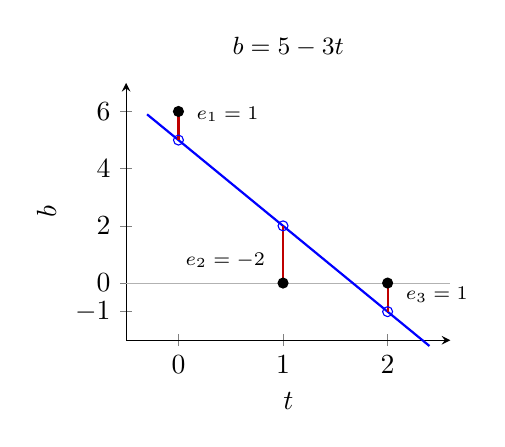
\begin{tikzpicture}
    \begin{axis}[width=0.47\textwidth,height=0.4\textwidth,xmin=-0.5,xmax=2.6,ymin=-2,ymax=7,
        xlabel={$t$},ylabel={$b$},axis lines=left,xtick={0,1,2},ytick={-1,0,2,4,6},
        title={\small $b=5-3t$},clip=false]
      \draw[gray!60] (axis cs:-0.5,0) -- (axis cs:2.6,0);
      \addplot[thick,blue,domain=-0.3:2.4] {5-3*x};
      \draw[red!75!black,thick] (axis cs:0,6) -- (axis cs:0,5);
      \draw[red!75!black,thick] (axis cs:1,0) -- (axis cs:1,2);
      \draw[red!75!black,thick] (axis cs:2,0) -- (axis cs:2,-1);
      \addplot[only marks,mark=*,mark size=1.8pt] coordinates {(0,6) (1,0) (2,0)};
      \addplot[only marks,mark=o,mark size=1.8pt,blue] coordinates {(0,5) (1,2) (2,-1)};
      \node[anchor=west,font=\scriptsize] at (axis cs:0.08,5.9) {$e_1=1$};
      \node[anchor=east,font=\scriptsize] at (axis cs:0.92,0.8) {$e_2=-2$};
      \node[anchor=west,font=\scriptsize] at (axis cs:2.08,-0.4) {$e_3=1$};
    \end{axis}
  \end{tikzpicture}
  \caption{The data picture of two least-squares fits. Dots are the data $b_i$, circles the
  heights $p_i$ of the best line, red segments the vertical errors $e_i=b_i-p_i$. Left: the
  lecture's points; right: the points $(0,6),(1,0),(2,0)$ with errors $(1,-2,1)$. The right
  angle of least squares is not visible here; it lives in $\R^3$, between $\vb{e}$ and the
  column space.}
  \label{fig:u18-fits}
\end{figure}

\begin{trap}
Least squares does \emph{not} minimize the perpendicular distances from the points to the
line. It minimizes the sum of squared \emph{vertical} errors $e_i=b_i-(C+Dt_i)$, because those
are the components of $A\vb{x}-\vb{b}$. The right angle is between $\vb{e}$ and $\Col{A}$ in
$\R^m$, not between the error segments and the line in the $t$--$b$ plane. A second warning:
squaring makes a single wild measurement (an \emph{outlier}) count heavily, so one bad point can
swing the whole line; statisticians check for outliers before trusting a least-squares fit.
\end{trap}

\subsection{When the normal equations can be solved}

Everything above assumed that $A\T A$ is invertible.

\begin{theorem}\label{thm:u18-invertible}
If $A$ has independent columns, then $A\T A$ is invertible.
\end{theorem}

\begin{proof}
Suppose $A\T A\vb{x}=\vb{0}$; we show $\vb{x}=\vb{0}$. Multiply by $\vb{x}\T$:
$\vb{x}\T A\T A\vb{x}=(A\vb{x})\T(A\vb{x})=\|A\vb{x}\|^2=0$, so $A\vb{x}=\vb{0}$. Independent
columns mean the only solution of $A\vb{x}=\vb{0}$ is $\vb{x}=\vb{0}$. So $\Nul{A\T A}=\{\vb{0}\}$
and the square matrix $A\T A$ is invertible. (This is half of the equality
$\Nul{A\T A}=\Nul{A}$ of Section~\ref{sec:u16}.)
\end{proof}

For a line fit, the columns $(1,\dots,1)$ and $(t_1,\dots,t_m)$ are independent as soon as two
of the $t_i$ differ, so least squares always has a unique line unless all measurements are at
the same time. Columns are certainly independent when they are \emph{orthonormal}:
perpendicular unit vectors such as $(1,0,0),(0,1,0),(0,0,1)$, or $(\cos\theta,\sin\theta)$ and
$(-\sin\theta,\cos\theta)$. Then $A\T A=I$ and the normal equations need no solving at all.
Section~\ref{sec:u19} shows how to make the columns orthonormal.

Nothing in the method needs the model to be a straight line; it only needs the unknown
coefficients to enter \emph{linearly}. A parabola $C+Dt+Et^2$ gives a matrix with columns $1$,
$t_i$, $t_i^2$; a curve through the origin $ct+dt^2$ gives columns $t_i$ and $t_i^2$
(Exercise~\ref{ex:u18-quad}).

\subsection{Exercises}

\begin{exercise}\label{ex:u18-ex1}
Write down three equations for the line $b=C+Dt$ to go through $b=7$ at $t=-1$, $b=7$ at
$t=1$, and $b=21$ at $t=2$. Find the least-squares solution $\hat{\vb{x}}=(C,D)$, the
projection $\vb{p}=A\hat{\vb{x}}$, and the error $\vb{e}$. Why is $P\vb{e}=\vb{0}$?
\end{exercise}

\begin{solution}
The equations are $C-D=7$, $C+D=7$, $C+2D=21$, so
\[
  A=\begin{bmatrix}1&-1\\1&1\\1&2\end{bmatrix},\quad
  A\T A=\begin{bmatrix}3&2\\2&6\end{bmatrix},\quad
  A\T\vb{b}=\begin{bmatrix}35\\42\end{bmatrix}.
\]
Solving $3C+2D=35$, $2C+6D=42$: three times the first minus the second gives $7C=63$, so
$C=9$ and $D=4$. The closest line is $b=9+4t$, with heights $\vb{p}=(5,13,17)$ and error
$\vb{e}=\vb{b}-\vb{p}=(2,-6,4)$. Since $\vb{e}\in\Nul{A\T}$ (check: $2-6+4=0$ and
$-2-6+8=0$), Proposition~\ref{prop:u18-extremes} gives $P\vb{e}=\vb{0}$; equivalently
$P\vb{e}=P\vb{b}-P\vb{p}=\vb{p}-\vb{p}=\vb{0}$.
\end{solution}

\begin{exercise}\label{ex:u18-ex2}
With the same times $t=-1,1,2$: (a) If the measurements are $\vb{b}=(2,-6,4)$, find
$\hat{\vb{x}}$ and the closest line. (b) If they are $\vb{b}=(5,13,17)$, find $\hat{\vb{x}}$
and $\vb{e}$. (c) Which of the four subspaces contain $\vb{e}$, $\vb{p}$, $\hat{\vb{x}}$? What
is $\Nul{A}$?
\end{exercise}

\begin{solution}
(a) This $\vb{b}$ is the previous error, which is perpendicular to $\Col{A}$; so
$A\T\vb{b}=\vb{0}$, $\hat{\vb{x}}=(0,0)$, $\vb{p}=\vb{0}$, and the best line is $b=0$.
(b) This $\vb{b}$ is the previous projection, which lies in $\Col{A}$; so
$\hat{\vb{x}}=(9,4)$ fits exactly and $\vb{e}=\vb{0}$.
(c) $\vb{e}\in\Nul{A\T}$, $\vb{p}\in\Col{A}$, $\hat{\vb{x}}\in\Col{A\T}=\R^2$ (the row space
is all of $\R^2$ here), and $\Nul{A}=\{\vb{0}\}$ because the columns are independent.
\end{solution}

\begin{exercise}\label{ex:u18-ex3}
Find the best line $C+Dt$ to fit $b=4,2,-1,0,0$ at times $t=-2,-1,0,1,2$.
\end{exercise}

\begin{solution}
The column of $t$'s is $(-2,-1,0,1,2)$, which is orthogonal to the column of ones (the times
are symmetric about $0$), so $A\T A$ is diagonal:
\[
  A\T A=\begin{bmatrix}5&0\\0&10\end{bmatrix},\qquad
  A\T\vb{b}=\begin{bmatrix}4+2-1+0+0\\-8-2+0+0+0\end{bmatrix}=\begin{bmatrix}5\\-10\end{bmatrix}.
\]
Hence $C=1$, $D=-1$, and the best line is $b=1-t$. Its errors are $(1,0,-2,0,1)$, which are
orthogonal to both columns.
\end{solution}

\begin{exercise}\label{ex:u18-short-practice}
Fit a least-squares line through $(0,0)$, $(1,3)$, $(2,0)$. What are $C$ and $D$?
\end{exercise}

\begin{solution}
The matrix is the same as in Example~\ref{ex:u18-short}, so $A\T A=\begin{bmatrix}3&3\\3&5\end{bmatrix}$,
and now $A\T\vb{b}=(3,3)$. The equations $3C+3D=3$ and $3C+5D=3$ give $D=0$, $C=1$: the flat
line $b=1$, with errors $(-1,2,-1)$, again a multiple of $(1,-2,1)$.
\end{solution}

\begin{exercise}\label{ex:u18-quad}
Find the curve $y=ct+dt^2$ through the origin that best fits $(1,1)$, $(2,5)$, $(-1,-2)$ in
the least-squares sense.
\end{exercise}

\begin{solution}
Plugging each point into $ct+dt^2=y$ gives
\[
  A=\begin{bmatrix}1&1\\2&4\\-1&1\end{bmatrix},\qquad
  \vb{x}=\begin{bmatrix}c\\d\end{bmatrix},\qquad
  \vb{b}=\begin{bmatrix}1\\5\\-2\end{bmatrix},
\]
with columns $t_i$ and $t_i^2$. Then
\[
  A\T A=\begin{bmatrix}1+4+1&1+8-1\\1+8-1&1+16+1\end{bmatrix}=\begin{bmatrix}6&8\\8&18\end{bmatrix},\qquad
  A\T\vb{b}=\begin{bmatrix}1+10+2\\1+20-2\end{bmatrix}=\begin{bmatrix}13\\19\end{bmatrix}.
\]
The determinant is $6\cdot 18-8\cdot 8=44$, and solving gives $c=\frac{13\cdot 18-8\cdot 19}{44}=\frac{41}{22}$,
$d=\frac{6\cdot 19-8\cdot 13}{44}=\frac{5}{22}$. The best curve is
$y=\frac{41}{22}t+\frac{5}{22}t^2$, with errors $\vb{e}=\frac{1}{11}(-12,4,-4)$; check that
$A\T\vb{e}=\vb{0}$. (If you watch the recitation video for this problem, note that the
$(2,2)$ entry of $A\T A$ is $1+16+1=18$; using $10$ there leads to a curve whose squared error,
$56$, is far larger than the true minimum $\frac{16}{11}$.)
\end{solution}
